\section{What we learned}\label{sec:learned}
\paragraph{The path matters, and which path depends on the family.} For squares in a square, hardening's lowest size is the lowest of all methods on \CsevenSquInSquHardenLowest{} of \CsevenSquInSquN{} instances and the only one that low on \CsevenSquInSquHardenSole{}; with identical settings, rigid starts manage \CsevenSquInSquRigidLowest{}. In 32 runs each, hardening alone reaches Trump's $n=11$ and Wainwright's $n=19$ packings (Figure~\ref{fig:strip}). For triangles the order reverses: rigid starts are lowest on \CsevenTriInSquRigidLowest{} instances of triangles in a square against \CsevenTriInSquHardenLowest{} for hardening, and \CsevenTriInTriRigidLowest{} against \CsevenTriInTriHardenLowest{} in a triangle (Figure~\ref{fig:tristrip}). On the control family the gradient paths reach the lowest size on the same number of instances, as they should.

\begin{figure}[t]\centering
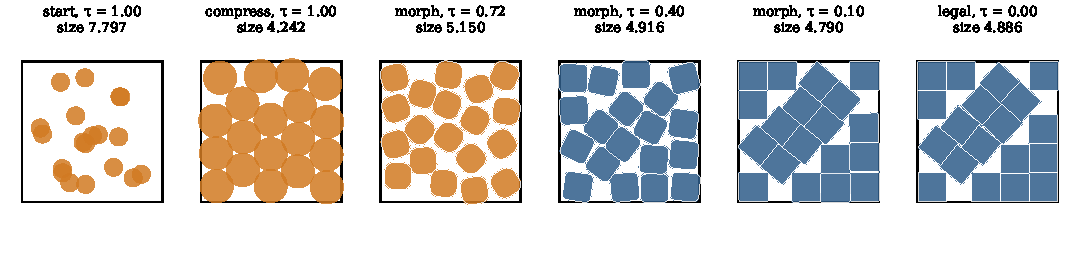
\includegraphics[width=\linewidth]{figures/strip_squ19}
\caption{One hardening run for 19 squares (C07): disks are compressed, harden into squares, and settle into Wainwright's packing (side $3+4\sqrt2/3$). Every replay is on the project site.}\label{fig:strip}
\end{figure}

\begin{figure}[t]\centering
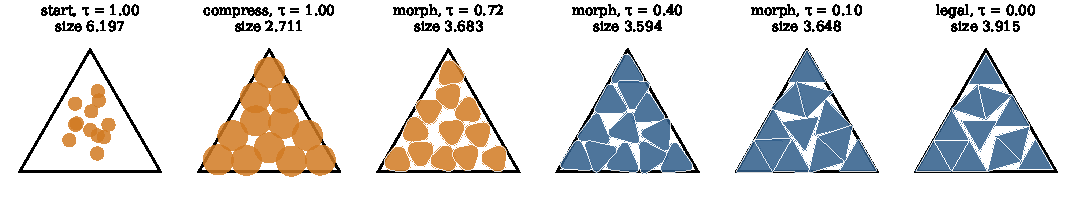
\includegraphics[width=\linewidth]{figures/strip_tri12}
\caption{The best of 32 hardening runs for 12 triangles in a triangle (C07) ends at $3.915$; rigid and snap starts reach the best known $3.879$. The disks settle into a near-hexagonal arrangement and the triangles that emerge from it keep orientations that do not tile.}\label{fig:tristrip}
\end{figure}

\paragraph{It is the gradual path, not the disk-compressed start.} Hardening differs from rigid starts in two ways: pieces are compressed as disks, and they then harden gradually. Campaign C11 separates the two with \emph{snap}, which compresses disks exactly as hardening does and then switches to the polygons in one step, with the same seeds, settings and budget (Table~\ref{tab:ablate}). We detect no difference between snap and rigid starts: over all \CsevenInstances{} instances each is lower than the other on \SnapRXLower{} and \SnapRRLower{} instances. Hardening differs from snap in both directions, by family: counting instances where hardening is lower against those where snap is lower, squares in a square give \SnapSquSqu{}, triangles in a triangle \SnapTriTri{} and triangles in a square \SnapTriSqu. The pre-registered test, over instances that exactly one of harden and snap solves, is \SnapHOnly{} against \SnapXOnly{} ($p=\SnapPReached$) over all families and inconclusive on squares in a square alone, where only two instances are discordant; the counts of lower sizes are clearer (harden \SnapHLower, snap \SnapXLower, $p=\SnapP$). The plan's rule says that if this test does not separate harden and snap on squares in a square, hardening's advantage there is attributed to the disk-compressed start. The test does not separate them, so that is the pre-registered conclusion; we record it, and also that the rule was poorly chosen, since a sign test over two discordant instances cannot reach significance. The rest of the evidence, which is descriptive and was not the pre-registered test, points the other way: we detect no gain from a disk-compressed start alone, and the instances where hardening and snap differ split by family, in hardening's favour on squares and against it on triangles.

\paragraph{Nor does the area schedule account for it.} A hardening piece also grows, by up to 40\% of its area. Campaign C12 keeps rigid polygons but scales them so that their area follows hardening's schedule exactly (\emph{grow-area}). We again detect no difference from rigid starts (lower on \AreaRXLower{} and \AreaRRLower{} instances, $p=\AreaRP$), and hardening differs from it in the same directions as from snap: \AreaSquSqu{} on squares in a square and \AreaTriTri{} on triangles in a triangle (Table~\ref{tab:ablate}). Over all instances, harden against grow-area is \AreaHLower{} against \AreaXLower{} ($p=\AreaP$); under the pre-registered rule (C12 uses C11's) the test on squares in a square is again inconclusive. Neither ablation reproduces hardening's pattern, which makes the rounding of the pieces the likeliest explanation, but these experiments do not establish it.

\begin{table}[t]\centering\small
\begin{tabular}{lrcccc}
\toprule
family & $N$ & harden : snap & snap : rigid & harden : grow-area & grow-area : rigid \\
\midrule
squares in square & 28 & 6 : 0 & 1 : 2 & 5 : 1 & 2 : 1 \\
squares in circle & 28 & 5 : 11 & 10 : 6 & 9 : 8 & 8 : 4 \\
squares in triangle & 29 & 0 : 1 & 0 : 0 & 0 : 1 & 0 : 0 \\
triangles in triangle & 28 & 0 : 8 & 0 : 2 & 1 : 8 & 0 : 3 \\
triangles in square & 28 & 6 : 14 & 8 : 9 & 5 : 11 & 5 : 6 \\
hexagons in square & 18 & 0 : 2 & 1 : 1 & 0 : 2 & 0 : 0 \\
disks in square & 29 & 0 : 0 & 0 : 0 & 0 : 0 & 0 : 0 \\
\midrule all & 188 & 17 : 36 & 20 : 20 & 20 : 31 & 15 : 14 \\
\bottomrule
\end{tabular}
\caption{Which part of hardening matters (C11, C12; harden and rigid from C07, same seeds, settings and budget). Each cell $a:b$ counts the instances on which the first method\textquotesingle s lowest size is lower than the second\textquotesingle s, and the reverse; the rest are ties. \emph{snap} compresses disks as hardening does, then switches to polygons at once; \emph{grow-area} keeps rigid polygons whose area follows hardening\textquotesingle s.}
\label{tab:ablate}
\end{table}


\paragraph{Why squares and not triangles?} We can only offer hypotheses. Along the path a piece's orientation matters in proportion to $1-\tau$ (Section~\ref{sec:method}), so hardening defers the choice of orientation until neighbours are nearly in place. Many of the best square packings, including $n=11$ and $19$, place a group of tilted squares between axis-aligned ones, where a late choice should help. The area explanation, that a triangle's inscribed disk covers only 60\% of it (a square's 79\%) and so a hardening triangle packing must grow and rearrange the most, is weakened by hexagons: their inscribed disk covers 91\%, yet hardening is no better than rigid starts there (lowest on \CsevenHexInSquHardenLowest{} against \CsevenHexInSquRigidLowest{} of \CsevenHexInSquN{} instances, mostly ties). A second hypothesis is orientational. Disks prefer a hexagonal arrangement; squares that emerge from it have four orientation classes and can tilt a little to fit, but good triangle packings alternate pieces pointing up and down, and a triangle's corners stick out twice as far as its inradius ($R/\rho=2$, against $\sqrt2$ for a square), so once corners appear a wrongly oriented triangle cannot turn without pushing its neighbours far apart. Figure~\ref{fig:tristrip} looks like this, but we did not test it.

\paragraph{Partly soft starts.} Varying only the starting softness $\tau_0$ on the \CtauN{} most contested instances (Table~\ref{tab:tau}), the counts of instances where each value reaches the lowest size are \CtauOne, \CtauHalf, \CtauQuarter{} and \CtauZero{} for $\tau_0=1, 0.5, 0.25, 0$. Squares in a square favour soft starts (\CtauSquares{}); triangles favour rigid or slightly rounded ones (\CtauTriangles{}). These instances were selected where hardening and rigid starts disagreed, mostly in rigid's favour, which tilts this count toward small $\tau_0$; partly rounded starts are a candidate default, not an established one.

\begin{table}[t]\centering\small
\begin{tabular}{lrrrrr}
\toprule
family & instances & $\tau_0=1$ (harden) & $0.5$ & $0.25$ & $0$ (rigid)\\
\midrule
squares in square & 6 & 3 & 4 & 2 & 0\\
squares in circle & 13 & 2 & 3 & 6 & 5\\
squares in triangle & 1 & 0 & 1 & 1 & 1\\
triangles in triangle & 7 & 0 & 4 & 3 & 5\\
triangles in square & 12 & 2 & 3 & 5 & 5\\
hexagons in square & 1 & 0 & 0 & 1 & 1\\
\midrule
all & 40 & 7 & 15 & 18 & 17\\
\bottomrule
\end{tabular}
\caption{How soft the start must be (C08): on the 40 most contested instances of C07, the number of instances where each starting softness $\tau_0$ reaches the lowest size (32 runs each, all other settings equal; ties counted for every tied value).}
\label{tab:tau}
\end{table}


\paragraph{Longer runs, or more runs?} An earlier test (C09, appendix) suggested that hardening gains more than rigid starts from longer schedules, but it changed run length and restart count together and used instances chosen because the two paths disagreed. Campaign C13 repeats it cleanly on \BudN{} instances fixed in advance ($n=11,17,23,29$ per family; hexagons $n=8,12,16,20$), with 32 runs at three times the budget, and 96 runs at the base budget for the same total cost. Counting instances where hardening is lower against those where rigid starts are lower: \BudOneH{} against \BudOneR{} with 32 base runs ($p=\BudOneP$), \BudThreeH{} against \BudThreeR{} with 32 long runs, and \BudMoreH{} against \BudMoreR{} with 96 base runs. Longer runs improved rigid starts more than hardening (rigid lower than its base on \BudGainR{} instances and higher on \BudLossR; hardening \BudGainH{} and \BudLossH), and at equal cost, three times longer runs and three times as many runs did about equally well for both paths (\BudLvMLH{} against \BudLvMMH{} for hardening, \BudLvMLR{} against \BudLvMMR{} for rigid). The C09 result does not replicate; we withdraw it.

\paragraph{Two paths, or more runs of one?} The paths fail on different families, so running both might help. At equal total budget, 32 rigid runs plus 32 hardening runs solve \PortRigidHarden{} of the \CsevenInstances{} instances, against \PortRigidSixtyFour{} for 64 rigid runs and \PortRigidGrow{} for 32 rigid plus 32 growing runs (instances solved by exactly one of the first two: \PortSign, two-sided $p=\PortP$). We detected no benefit from mixing; at this size that does not show there is none, and whether mixing pays when the family is known to favour the second path was not tested.

\paragraph{Tuning decides comparisons.} Our first experiments compared hardening with rigid starts that inherited the hardening schedule, on two square instances, and hardening looked better. Tuned with comparable effort, rigid starts led overall. Re-tuning for the lowest point instead of the median changed four of the five methods' settings (stronger pressure for the gradient paths, more noise for rigid starts) and helped simulated annealing most. It kept the broad pattern, hardening for squares in a square and rigid or growing starts for triangles, though the leading method changed for squares in a circle and triangles in a square.
